\subsection{雪崩増幅}
半導体内の電場がある値を超えると、電子と正孔が雪崩増幅を起こす。図\ref{fg:avalance} はその過程を示したものになっている。
図\ref{fg:avalance} 中の1番の電子に注目すると、高電場によってこの電子の運動エネルギーが増加する。
この電子が格子に衝突した際に、持っていた運動エネルギーによって、格子の結合手を切断し、価電子帯から電子が励起される。
この過程によって生じた電子正孔対が2番の電子と$\rm{2^\prime}$番の正孔である。この電子と正孔も高電場によって、格子に衝突し、電子正孔対を生成する。
このように、高電場によって連鎖的に電子と正孔が生じる過程を電子雪崩(アバランシェ)という。

\begin{figure}[h]
    \centering
    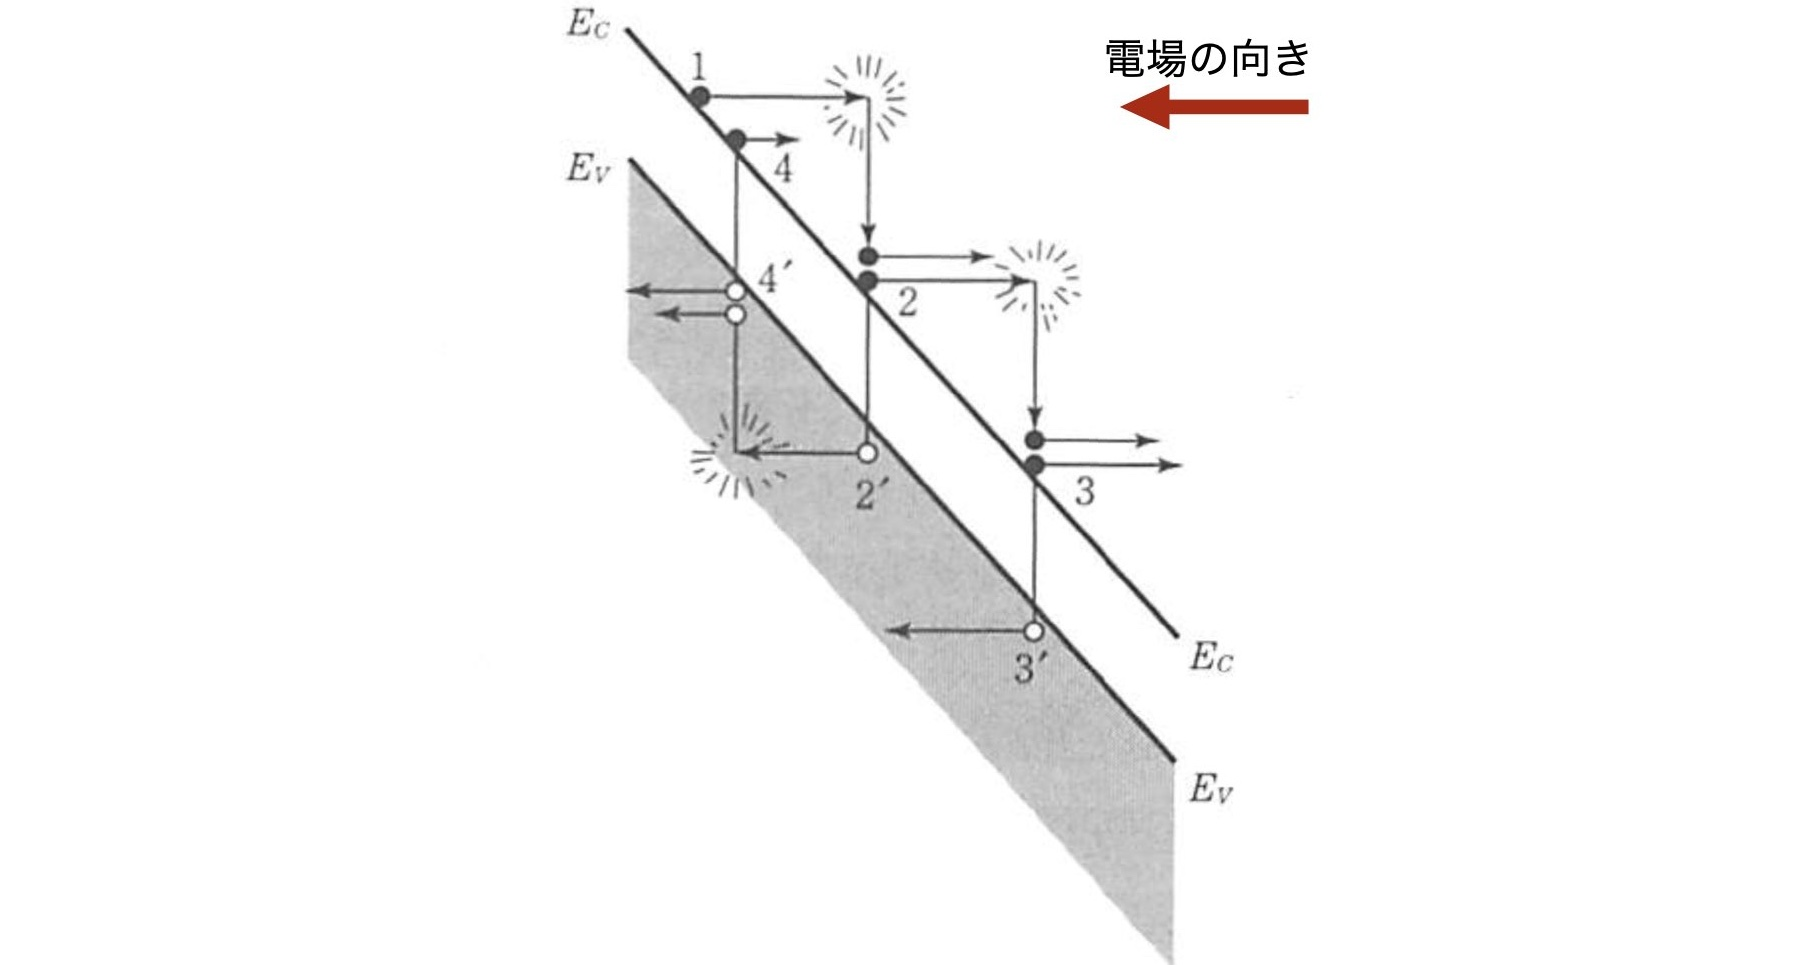
\includegraphics[width=11cm]{fig/ch3/avalance.jpeg}
    \caption[電子雪崩におけるエネルギーバンド図\cite{sze2012semiconductor}]{電子雪崩におけるエネルギーバンド図\cite{sze2012semiconductor}\\電子や正孔が衝突して電子正孔対を生成する現象が繰り返し生じる。}
    \label{fg:avalance}
\end{figure}

